\documentclass[10pt,a4paper]{article}
\usepackage[utf8]{inputenc}
\usepackage[T1]{fontenc}
\IfFileExists{spanish.ldf}{\usepackage[spanish,es-noshorthands]{babel}}{}
\usepackage[margin=1.8cm]{geometry}
\IfFileExists{enumitem.sty}{\usepackage{enumitem}\setlist{nosep,leftmargin=*}}{}
\usepackage{graphicx}
\usepackage{longtable}
\usepackage{array}
\usepackage[table]{xcolor}
\usepackage{pdflscape}
\usepackage{fancyhdr}
\usepackage{caption}
\usepackage{hyperref}
\captionsetup{font=small}
\definecolor{hdr}{HTML}{DCE6F1}
\hypersetup{colorlinks=true,urlcolor=blue!60!black,linkcolor=black,pdftitle={TA-IND-01: IEEE 29148 y tipos de requisitos},pdfauthor={Basurto Anchaguano Jordan Steven}}
\newcommand{\pend}{\textcolor{red}{[COMPLETAR]}}
\newcommand{\pendc}{\textcolor{red}{[\ldots]}}
\setlength{\parskip}{2pt}\linespread{0.95}\emergencystretch=2em
\pagestyle{fancy}\fancyhf{}
\lhead{\small TA-IND-01 \textperiodcentered{} ISR-401}
\rhead{\small Basurto Anchaguano Jordan Steven}
\cfoot{\small P\'agina \thepage}
\renewcommand{\refname}{Referencias}
\begin{document}

{\LARGE\bfseries TA-IND-01: IEEE 29148 y tipos de requisitos de un sistema conocido}\\[3pt]
{\large Ingenier\'ia de Requerimientos (ISR-401) \textperiodcentered{} UTEQ}

\medskip
\begin{tabular}{@{}ll}
\textbf{Estudiante:} & Basurto Anchaguano Jordan Steven\\
\textbf{Sistema analizado:} & Epic Games Store (launcher de escritorio)\\
\textbf{Fecha:} & 11 de noviembre de 2026\\
\textbf{Repositorio:} & \url{https://github.com/EleSteven777/ISR401-BasurtoJordan}\\
\end{tabular}

\section{Descripci\'on del sistema}
Epic Games Store se utiliza principalmente para reclamar los juegos gratuitos semanales, así como para descargar e iniciar títulos de la biblioteca, como Rocket League o Grand Theft Auto V. Esta plataforma es empleada cotidianamente por jugadores de PC, tanto casuales como competitivos. Habitualmente, el sistema se ejecuta un par de veces por semana durante los ratos libres en una laptop con Windows, utilizando una conexión a una red Wi-Fi doméstica para descargar las actualizaciones de los videojuegos. En este contexto, el presente trabajo analiza específicamente el launcher de escritorio en lugar de la tienda web, ya que evaluar la aplicación local permite realizar mediciones reales y verificables en el equipo, tales como observar el consumo de memoria RAM o cronometrar los tiempos de carga.

\section{Resumen anal\'itico de la norma ISO/IEC/IEEE 29148:2018}
Este resumen y el resto del informe siguen lo solicitado en la gu\'ia de la actividad~\cite{guia}.

\subsection{Requisito bien formado (cl\'ausula 5.2.4)}
Un requisito se arma con un sujeto (el sistema), un verbo que obliga («shall», que en los requisitos del launcher se expresó como «debe»), la acción o capacidad que se pide y las condiciones que la limitan. La norma usa «should» para lo recomendable, «may» para lo opcional y «will» para hechos, y aconseja no usar «must» porque se presta a confusión. Por ejemplo, en R01 el sujeto es «el launcher», el verbo es «debe mostrar», la acción es «la pantalla de inicio de la tienda» y la condición es «en un máximo de 5,0 s desde el clic en el icono»~\cite[cl.~5.2.4]{iso29148}.

\subsection{Caracter\'isticas de un requisito individual (cl\'ausula 5.2.5)}
La norma establece nueve caracter\'isticas para cada requisito \cite[cl.~5.2.5]{iso29148}:
\begin{enumerate}
\item \textbf{Necessary (necesario):} si se quita, el sistema queda con algo que le falta. R02: sin él, nada limita la RAM que gasta el launcher minimizado.
\item \textbf{Appropriate (apropiado):} tiene el nivel de detalle justo y no decide el diseño interno. R13: pide iniciar el juego con 1 clic, pero no dice cómo programarlo.
\item \textbf{Unambiguous (inequívoco):} solo se puede entender de una forma. R01: dice exactamente cuándo empieza y cuándo termina la medición.
\item \textbf{Complete (completo):} se entiende solo, sin buscar información en otra parte. R06: incluye la pestaña y que no haya descargas activas; la herramienta de medición está en su criterio de aceptación.
\item \textbf{Singular (singular):} habla de una sola cosa. R09: trata un solo filtro («Instalados») con un solo efecto.
\item \textbf{Feasible (factible):} se puede cumplir con lo que hay. R08: el primer borrador pedía que todo funcionara sin internet, y eso no se puede; la versión corregida pide solo el aviso de sin conexión.
\item \textbf{Verifiable (verificable):} hay una forma concreta de comprobarlo. R02: se midió en el Administrador de Tareas y dio 179,8 MB, por debajo de 200 MB.
\item \textbf{Correct (correcto):} refleja lo que de verdad se necesita y lo que hace el sistema. R05: se corrigió porque, con la pestaña «Biblioteca» abierta, la primera opción sigue en inglés («Store») aunque el idioma esté en español.
\item \textbf{Conforming (conforme):} sigue el formato acordado. R12: usa la misma estructura que los demás: «El launcher debe + acción + condición».
\end{enumerate}

\subsection{Caracter\'isticas de un conjunto de requisitos (cl\'ausula 5.2.6)}
El conjunto debe cumplir cinco caracter\'isticas \cite[cl.~5.2.6]{iso29148}:
\begin{enumerate}
\item \textbf{Complete (completo):} al conjunto no le faltan partes ni tiene nada «por definir». Ejemplo: los 15 requisitos cubren la tienda, la biblioteca, las descargas, el desempeño y la interfaz.
\item \textbf{Consistent (consistente):} los requisitos no se contradicen y cada cosa tiene siempre el mismo nombre. Ejemplo: se usa siempre «Epic Games Launcher» para el proceso y «Biblioteca» para la pestaña.
\item \textbf{Feasible (factible):} todos juntos se pueden cumplir a la vez. Ejemplo: R02 (RAM $\leq$ 200 MB) y R06 (CPU $\leq$ 1,0 \%) se cumplieron en la misma laptop.
\item \textbf{Comprehensible (comprensible):} se entiende qué se espera del sistema. Ejemplo: cada requisito dice la pantalla y el botón exactos.
\item \textbf{Able to be validated (validable):} se puede demostrar que el conjunto cubre lo que necesita el usuario. Ejemplo: cada requisito tiene su criterio de aceptación con una medición.
\end{enumerate}

\subsection{T\'erminos que la norma proh\'ibe (cl\'ausula 5.2.7)}
La norma proh\'ibe estos tipos de t\'erminos \cite[cl.~5.2.7]{iso29148}:
\begin{itemize}
\item \textbf{Superlativos:} «el mejor», «el más rápido».
\item \textbf{Lenguaje subjetivo:} «fácil», «verse bien».
\item \textbf{Pronombres vagos:} «esto» o «eso» cuando no queda claro a qué se refieren.
\item \textbf{Adjetivos y adverbios ambiguos:} «rápidamente», «mucha», «adecuada».
\item \textbf{Términos abiertos:} «dar soporte», «pero no limitado a».
\item \textbf{Comparaciones:} «mejor que», «de mayor calidad».
\item \textbf{Salidas de escape:} «si es posible», «según corresponda».
\item \textbf{Palabras de totalidad:} «todos», «siempre», «nunca», «cualquier». R11 antes de corregirlo («antes de iniciar cualquier descarga»).
\item \textbf{Referencias incompletas:} cerrar una lista con «etc.».
\end{itemize}

\section{Glosario de 10 t\'erminos de la cl\'ausula 3}
La Tabla~\ref{tab:glosario} presenta diez t\'erminos de la cl\'ausula 3 de la norma~\cite{iso29148}, cada uno con su definici\'on parafraseada y un ejemplo tomado del launcher de Epic Games.

\begingroup\scriptsize\setlength{\tabcolsep}{2.5pt}\renewcommand{\arraystretch}{1.05}
\begin{longtable}{|>{\raggedright\arraybackslash}p{0.8cm}|>{\raggedright\arraybackslash}p{3.4cm}|>{\raggedright\arraybackslash}p{1.4cm}|>{\raggedright\arraybackslash}p{5.8cm}|>{\raggedright\arraybackslash}p{3.4cm}|}
\caption{Glosario de términos de la cláusula 3.}\label{tab:glosario}\\
\hline\rowcolor{hdr}\textbf{N.°} & \textbf{Término} & \textbf{Cláusula} & \textbf{Definición parafraseada} & \textbf{Ejemplo en el sistema} \\ \hline
\endfirsthead
\hline\rowcolor{hdr}\textbf{N.°} & \textbf{Término} & \textbf{Cláusula} & \textbf{Definición parafraseada} & \textbf{Ejemplo en el sistema} \\ \hline
\endhead
1 & Acquirer (adquiriente) & 3.1.1 & Quien compra u obtiene un producto o servicio de un proveedor. & Yo, cuando reclamo el juego gratis de la semana en la tienda de Epic. \\ \hline
2 & Attribute (atributo) & 3.1.2 & Una característica de algo que se puede medir o describir. & El tamaño de descarga de GTA V (116 GB) o su estado «Instalado» en la biblioteca. \\ \hline
3 & Baseline (línea base) & 3.1.3 & Una versión aprobada que se toma de referencia y solo cambia si se aprueba el cambio. & La lista final de mis 15 requisitos corregidos, que ya no se cambia sin justificarlo. \\ \hline
4 & Concept of operations (concepto de operaciones) & 3.1.5 & La idea general de cómo una organización piensa usar el sistema. & Mi uso normal es abrir el launcher un par de veces por semana, reclamar el juego gratis en «Store», instalar desde «Biblioteca» lo que quiero y jugar Rocket League o GTA V. \\ \hline
5 & Condition (condición) & 3.1.6 & Algo medible que se le pone al requisito para decir cuándo o cuánto debe cumplirse. & En R02, medir la RAM «con el launcher minimizado durante un minuto». \\ \hline
6 & Constraint (restricción) & 3.1.7 & Un límite que viene de afuera y que el sistema o su diseño tienen que respetar. & El launcher tiene que funcionar en Windows 11 y proponer la ruta C:\textbackslash{}Program Files\textbackslash{}Epic Games. \\ \hline
7 & Context of use (contexto de uso) & 3.1.8 & Quién usa el sistema, para qué, con qué equipo y en qué ambiente. & Un estudiante que juega Rocket League en sus ratos libres, en una laptop con Wi-Fi de la casa. \\ \hline
8 & Customer (cliente) & 3.1.9 & La persona u organización que recibe el producto o servicio. & Cualquier jugador que recibe la descarga de un juego desde la tienda. \\ \hline
9 & Derived requirement (requisito derivado) & 3.1.10 & Un requisito que nadie pidió directamente pero que sale de otros requisitos. & Como R14 propone instalar por defecto en C:\textbackslash{}Program Files\textbackslash{}Epic Games\textbackslash{} y R11 muestra que GTA V ocupa 116 GB, de ahí sale que el launcher debe avisar si en la unidad C: no hay espacio libre suficiente antes de empezar la instalación. \\ \hline
10 & Operational scenario (escenario operacional) & 3.1.17 & Una secuencia de pasos imaginada que muestra cómo se usaría el sistema. & Abro el launcher, entro a «Biblioteca», hago clic en GTA V, elijo la carpeta y empieza la descarga. \\ \hline
\end{longtable}
\endgroup

\begin{landscape}
\section{Requisitos formulados y clasificaci\'on}
La Tabla~\ref{tab:requisitos} reúne los 15 requisitos formulados para el launcher y su clasificación; los de calidad se asignan con ISO/IEC 25010:2023~\cite{iso25010}.

\begingroup\scriptsize\setlength{\tabcolsep}{2.5pt}\renewcommand{\arraystretch}{1.05}
\begin{longtable}{|>{\raggedright\arraybackslash}p{1cm}|>{\raggedright\arraybackslash}p{2.1cm}|>{\raggedright\arraybackslash}p{6.6cm}|>{\raggedright\arraybackslash}p{3.4cm}|>{\raggedright\arraybackslash}p{2.6cm}|>{\raggedright\arraybackslash}p{9.2cm}|}
\caption{Requisitos formulados, clasificación y criterio de aceptación.}\label{tab:requisitos}\\
\hline\rowcolor{hdr}\textbf{ID} & \textbf{Tipo} & \textbf{Enunciado} & \textbf{Característica ISO/IEC 25010:2023 (si es de calidad)} & \textbf{Métrica y umbral} & \textbf{Criterio de aceptación} \\ \hline
\endfirsthead
\hline\rowcolor{hdr}\textbf{ID} & \textbf{Tipo} & \textbf{Enunciado} & \textbf{Característica ISO/IEC 25010:2023 (si es de calidad)} & \textbf{Métrica y umbral} & \textbf{Criterio de aceptación} \\ \hline
\endhead
R01 & Desempeño / Calidad & El launcher de Epic Games debe mostrar la pantalla de inicio de la tienda en un máximo de 5,0 s, contados desde el clic en el icono del launcher cerrado por completo, en una laptop con Windows 11, procesador AMD Ryzen 5 5625U y 16 GB de RAM conectada a una red Wi-Fi doméstica. & Eficiencia de desempeño (performance efficiency); comportamiento temporal (time behaviour), 3.2.1 & Tiempo de respuesta $\leq$ 5,0 s & Cerrar el launcher por completo, abrirlo y cronometrar desde el clic hasta que se ve la pantalla de inicio; 3 repeticiones, todas $\leq$ 5,0 s. Medido el 11/11/2026 a las 19:15: 4,31 s, 4,68 s y 4,16 s. \\ \hline
R02 & Desempeño / Calidad & El proceso «Epic Games Launcher» debe consumir un máximo de 200 MB de memoria RAM, medido en el Administrador de Tareas de Windows con el launcher minimizado durante un minuto. & Eficiencia de desempeño (performance efficiency); utilización de recursos (resource utilization), 3.2.2 & Consumo de memoria RAM $\leq$ 200 MB & Con el launcher minimizado durante 1 minuto, leer la columna «Memoria» del proceso «Epic Games Launcher» en el Administrador de Tareas; valor $\leq$ 200 MB. Medido el 11/11/2026 a las 19:20: 179,8 MB. \\ \hline
R03 & Usabilidad / Calidad & El launcher debe permitir pausar una descarga en curso en un máximo de 2 clics: uno en el icono de descargas ubicado abajo a la izquierda y otro en el botón de pausa. & Capacidad de interacción (interaction capability); operabilidad (operability), 3.4.3 & Número de clics $\leq$ 2 & Con una descarga en curso, contar los clics desde el icono de descargas situado abajo a la izquierda hasta pausarla; valor $\leq$ 2 clics. Medido el 11/11/2026 a las 19:25: 2 clics. \\ \hline
R04 & Funcional & El buscador de la tienda debe desplegar la lista de sugerencias tras ingresar un máximo de 4 caracteres en la barra de búsqueda superior. & --- & --- & Escribir caracteres uno por uno en la barra de búsqueda y contar cuántos se requieren para que aparezca el listado; el límite se fija en 4 caracteres para cubrir títulos de 3 y 4 letras iniciales. Medido el 11/11/2026 a las 19:35: al escribir «GTA» desplegó sugerencias al 3.er carácter; al escribir «Fall» desplegó sugerencias al 4.º carácter. \\ \hline
R05 & Funcional & El launcher debe mostrar el texto «Biblioteca» en el menú lateral izquierdo cuando el idioma seleccionado en «Ajustes» es «Español». & --- & --- & Seleccionar el idioma español en ajustes, reiniciar el launcher y comprobar en el menú lateral izquierdo que la opción muestre «Biblioteca» (con la pestaña «Biblioteca» abierta, la primera opción aparece como «Store»; con la pestaña de la tienda abierta aparece como «Tienda»). Medido el 11/11/2026 a las 19:38: verificado en pantalla. \\ \hline
R06 & Desempeño / Calidad & El proceso «Epic Games Launcher» debe consumir un máximo del 1,0 \% de uso de CPU medido en la laptop con el launcher abierto en primer plano en la pestaña «Biblioteca» y sin descargas activas. & Eficiencia de desempeño (performance efficiency); utilización de recursos (resource utilization), 3.2.2 & Uso de CPU $\leq$ 1,0 \% & Con el launcher abierto en la laptop en la pestaña «Biblioteca», observar la columna «CPU» del proceso «Epic Games Launcher» en el Administrador de Tareas durante 30 segundos; valor $\leq$ 1,0 \%. Medido el 11/11/2026 a las 19:41: valores entre 0,1 \% y 0,3 \%. \\ \hline
R07 & Funcional & El launcher debe ocultar su ventana principal manteniendo el proceso «Epic Games Launcher» activo en segundo plano al hacer clic en el botón cerrar «X» de la esquina superior derecha. & --- & --- & Hacer clic en el botón «X» de la ventana y comprobar en la pestaña «Procesos» del Administrador de Tareas que «Epic Games Launcher» permanece en ejecución. Medido el 11/11/2026 a las 19:43: ventana oculta y proceso activo. \\ \hline
R08 & Funcional & El launcher debe mostrar un aviso de sin conexión en la pestaña «Store» cuando se ejecuta en la laptop con el Wi-Fi desactivado. & --- & --- & Desactivar el Wi-Fi de la laptop, abrir el launcher y comprobar que no carga el catálogo de la tienda y muestra el aviso de falta de conexión. Medido el 11/11/2026 a las 19:46: bloqueo del catálogo verificado en pantalla. \\ \hline
R09 & Funcional & El launcher debe ocultar de la cuadrícula de juegos aquellos títulos no instalados al activar el filtro «Instalados» en la pestaña «Biblioteca». & --- & --- & En la pestaña «Biblioteca», marcar el filtro «Instalados» y comprobar visualmente que solo permanecen en la cuadrícula los juegos ya instalados en el disco. Medido el 11/11/2026 a las 19:48: lista reducida únicamente a juegos instalados. \\ \hline
R10 & Usabilidad / Calidad & El launcher debe desplegar exactamente 1 cuadro de diálogo de confirmación antes de borrar los archivos tras seleccionar «Desinstalar» en el menú de opciones de un juego instalado. & Capacidad de interacción (interaction capability); protección contra errores de usuario (user error protection), 3.4.4 & Confirmaciones previas al borrado = 1 cuadro de diálogo & Abrir el menú de tres puntos de un juego instalado, hacer clic en «Desinstalar» y contar los cuadros de confirmación que aparecen antes de que inicie el borrado; valor = 1. Medido el 11/11/2026 a las 19:50: aparece 1 cuadro de diálogo con el botón «Desinstalar». \\ \hline
R11 & Funcional & El launcher debe mostrar el tamaño de descarga en gigabytes (GB) al seleccionar el título «Grand Theft Auto V» para su instalación desde la biblioteca. & --- & --- & Hacer clic sobre el título no instalado «Grand Theft Auto V» en la biblioteca y leer el valor del espacio requerido en pantalla. Medido el 11/11/2026 a las 19:53: muestra «116 GB». \\ \hline
R12 & Funcional & El launcher debe eliminar una descarga en curso de la vista de descargas (donde se muestran las secciones «Descripción general» y «Actividad reciente») al hacer clic en el botón «Cancelar» (icono «X»). & --- & --- & Con una descarga en curso, abrir la vista de descargas desde el icono inferior izquierdo, pulsar el botón «Cancelar» y comprobar que la descarga activa se detiene y desaparece. Medido el 11/11/2026 a las 19:55: descarga eliminada. \\ \hline
R13 & Usabilidad / Calidad & El launcher debe iniciar la ejecución de un juego instalado en un máximo de 1 clic sobre su carátula dentro de la pestaña «Biblioteca». & Capacidad de interacción (interaction capability); operabilidad (operability), 3.4.3 & Número de clics $\leq$ 1 & En la pestaña «Biblioteca», hacer clic izquierdo sobre la carátula de un juego instalado y contar los clics necesarios para que el estado bajo la carátula cambie a «Iniciando»; valor $\leq$ 1 clic. Medido el 11/11/2026 a las 19:57: 1 clic, el texto inferior cambió a «Iniciando». \\ \hline
R14 & Restricción de diseño & El launcher debe proponer por defecto la ruta base C:\textbackslash{}Program Files\textbackslash{}Epic Games\textbackslash{} en el campo «Carpeta» de la ventana «Elegir ubicación de instalación» en Windows 11. & --- & --- & Hacer clic en un juego no instalado en la biblioteca y comprobar en el cuadro «Elegir ubicación de instalación» que la ruta inicial comience con C:\textbackslash{}Program Files\textbackslash{}Epic Games\textbackslash{}. Medido el 11/11/2026 a las 19:58: ruta verificada en pantalla. \\ \hline
R15 & Interfaz & El launcher debe mostrar su ventana principal sin bordes negros ni recortes de contenido al maximizarse en un monitor externo con resolución de 1920 $\times$ 1080 píxeles a 100 Hz conectado por HDMI a la laptop. & --- & --- & Mover la ventana del launcher al monitor externo 1080p de 100 Hz conectado por HDMI, pulsar el botón «Maximizar» de Windows y comprobar visualmente que la ventana cubre los 1920 $\times$ 1080 píxeles sin bandas negras ni texto cortado. Medido el 11/11/2026 a las 20:00: sin bordes negros ni recortes. \\ \hline
\end{longtable}
\endgroup

\section{Capturas del sistema}
Las Figuras~\ref{fig:c1} a~\ref{fig:c3} muestran las pantallas del launcher sobre las que se formularon los requisitos.

\begin{center}
\begin{minipage}[t]{0.32\linewidth}\centering
\IfFileExists{figuras/captura1.png}{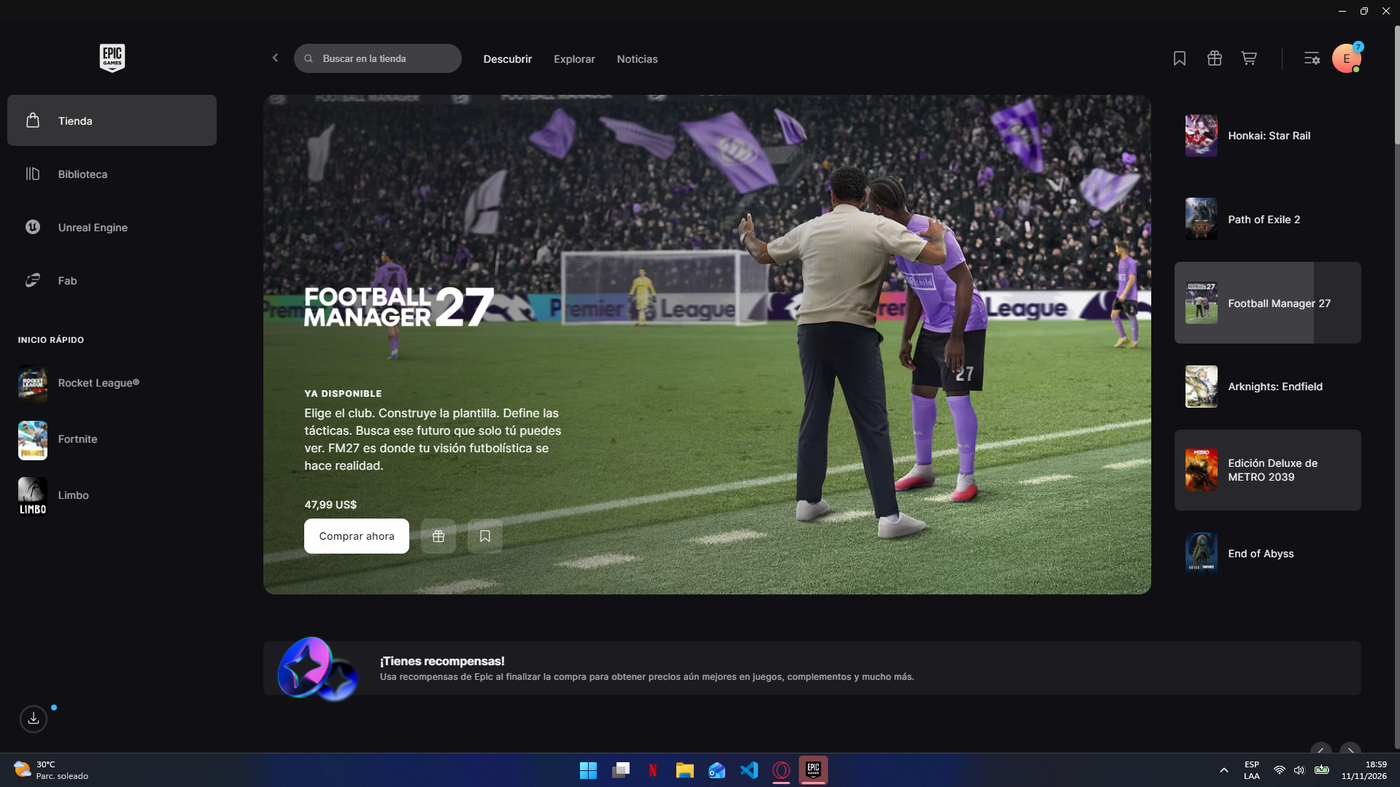
\includegraphics[width=\linewidth]{figuras/captura1.png}}{\fbox{\pend\ captura1.png}}
\captionof{figure}{Pantalla principal de la tienda del launcher.}\label{fig:c1}\end{minipage}\hfill
\begin{minipage}[t]{0.32\linewidth}\centering
\IfFileExists{figuras/captura2.png}{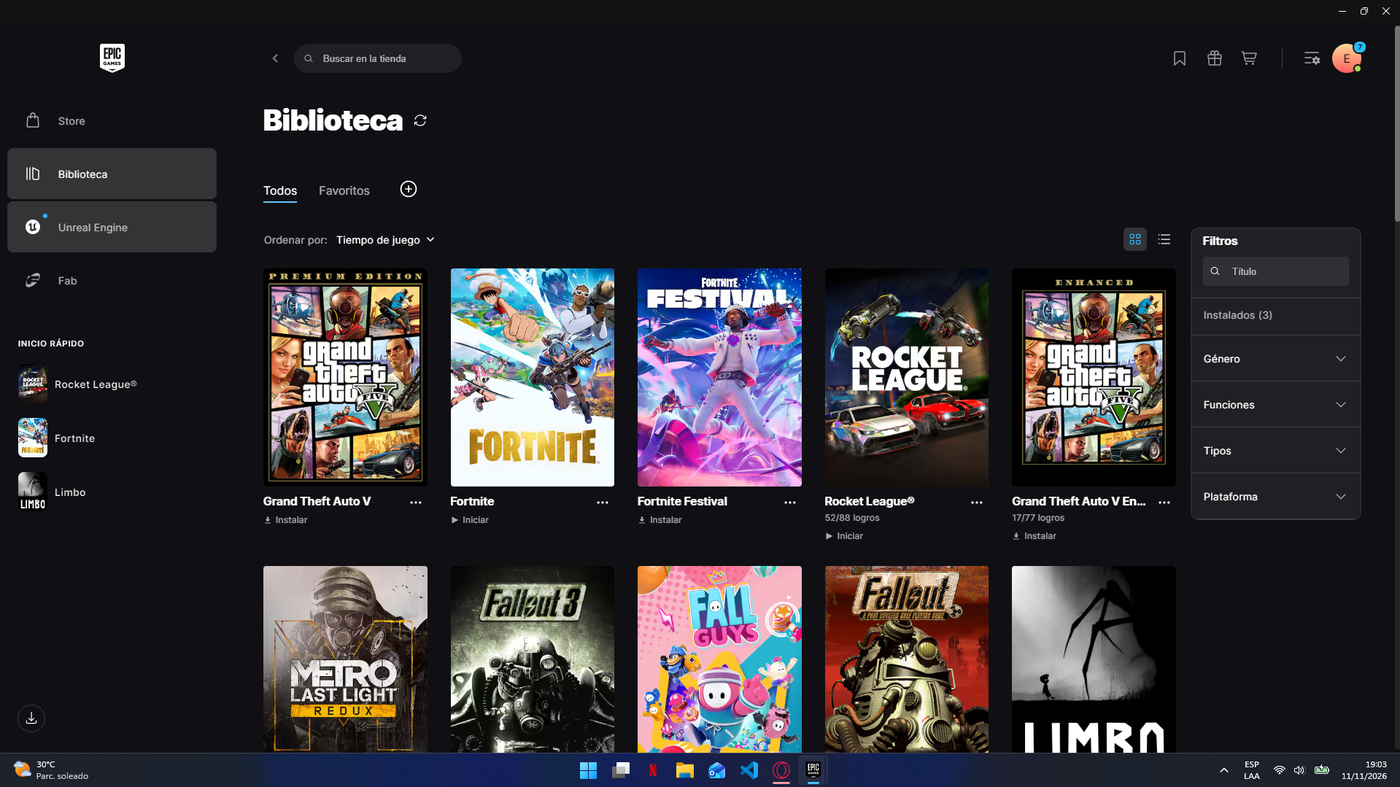
\includegraphics[width=\linewidth]{figuras/captura2.png}}{\fbox{\pend\ captura2.png}}
\captionof{figure}{Biblioteca del launcher.}\label{fig:c2}\end{minipage}\hfill
\begin{minipage}[t]{0.32\linewidth}\centering
\IfFileExists{figuras/captura3.png}{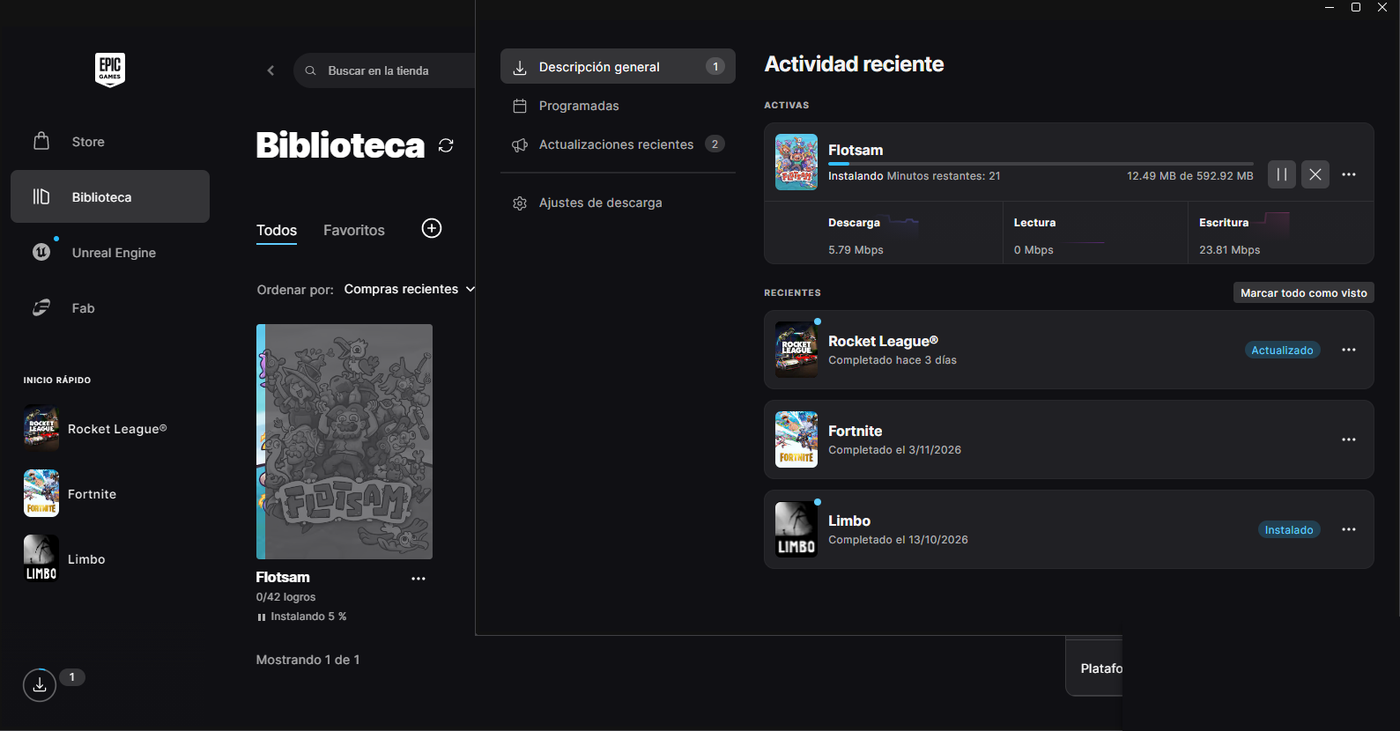
\includegraphics[width=\linewidth]{figuras/captura3.png}}{\fbox{\pend\ captura3.png}}
\captionof{figure}{Vista de descargas del launcher.}\label{fig:c3}\end{minipage}
\end{center}
\end{landscape}

\begin{landscape}
\section{Autoevaluaci\'on y versi\'on corregida}
La Tabla~\ref{tab:autoeval} compara la versi\'on anterior de cada requisito con la versi\'on corregida.

\begingroup\scriptsize\setlength{\tabcolsep}{2.5pt}\renewcommand{\arraystretch}{1.05}
\begin{longtable}{|>{\raggedright\arraybackslash}p{1cm}|>{\raggedright\arraybackslash}p{5.6cm}|>{\raggedright\arraybackslash}p{5.6cm}|>{\raggedright\arraybackslash}p{7.4cm}|>{\raggedright\arraybackslash}p{5.0cm}|}
\caption{Autoevaluación de los requisitos y versión corregida.}\label{tab:autoeval}\\
\hline\rowcolor{hdr}\textbf{ID} & \textbf{Versión anterior} & \textbf{Problema detectado (con la cláusula)} & \textbf{Versión corregida} & \textbf{Por qué mejora} \\ \hline
\endfirsthead
\hline\rowcolor{hdr}\textbf{ID} & \textbf{Versión anterior} & \textbf{Problema detectado (con la cláusula)} & \textbf{Versión corregida} & \textbf{Por qué mejora} \\ \hline
\endhead
R01 & El launcher debe abrir la tienda en un máximo de 5,0 s con el launcher cerrado por completo, en una laptop con Windows y Wi-Fi doméstico. & «Abrir la tienda» no dice cuándo empieza ni cuándo termina la medición: ¿al hacer clic, cuando aparece la ventana o cuando carga el catálogo? Además, «una laptop con Windows» no indica versión ni hardware, y el tiempo cambia según el equipo. Falla en ser inequívoco y completo (5.2.5) y no tiene una condición medible (5.2.1). & El launcher de Epic Games debe mostrar la pantalla de inicio de la tienda en un máximo de 5,0 s, contados desde el clic en el icono del launcher cerrado por completo, en una laptop con Windows 11, procesador AMD Ryzen 5 5625U y 16 GB de RAM conectada a una red Wi-Fi doméstica. & Ahora la medición empieza con el clic en el icono y termina cuando se ve la pantalla de inicio, y el equipo queda fijado (Windows 11, Ryzen 5 5625U, 16 GB). Por eso los 4,31 s, 4,68 s y 4,16 s se pueden repetir. \\ \hline
R02 & El proceso «Epic Games Launcher» debe consumir memoria RAM en un máximo de 200 MB estando minimizado. & «Estando minimizado» no dice con qué herramienta se mide ni cuánto hay que esperar después de minimizar. Como la RAM baja poco a poco, una lectura a los 5 segundos y otra al minuto dan valores distintos. Falla en ser verificable y completo (5.2.5). & El proceso «Epic Games Launcher» debe consumir un máximo de 200 MB de memoria RAM, medido en el Administrador de Tareas de Windows con el launcher minimizado durante un minuto. & Se agregó el instrumento (columna «Memoria» del Administrador de Tareas) y el tiempo de espera (un minuto), así que la lectura de 179,8 MB se obtiene de la misma forma. \\ \hline
R03 & El launcher debe pausar una descarga en un máximo de 2 clics con una descarga en curso, desde el icono de descargas. & «El launcher debe pausar… en 2 clics» pone al sistema a hacer los clics que hace el usuario, y eso rompe la estructura sujeto-acción de 5.2.4. Además, «el icono de descargas» no dice dónde está ni cuál es el segundo clic, así que no se sabe qué contar. Falla en ser inequívoco (5.2.5). & El launcher debe permitir pausar una descarga en curso en un máximo de 2 clics: uno en el icono de descargas ubicado abajo a la izquierda y otro en el botón de pausa. & Con «debe permitir» queda claro que es una capacidad del sistema, y ahora se nombran los dos clics que se cuentan: el icono de abajo a la izquierda y el botón de pausa. \\ \hline
R04 & El buscador de la tienda debe desplegar una lista predictiva de resultados tras ingresar un máximo de 3 caracteres en la barra superior. & el umbral de 3 caracteres no coincide con lo que hace el launcher. Al escribir «Fall», las sugerencias aparecieron recién en el 4.º carácter, así que con esta versión el requisito fallaría la prueba aunque el buscador funcione bien. No es correcto (5.2.5). Además, «la barra superior» no aclara que se trata de la barra de búsqueda de la tienda. & El buscador de la tienda debe desplegar la lista de sugerencias tras ingresar un máximo de 4 caracteres en la barra de búsqueda superior. & el umbral de 4 caracteres cubre los dos casos medidos («GTA» al 3.º y «Fall» al 4.º), y ahora se nombra la barra de búsqueda. \\ \hline
R05 & El launcher debe traducir los elementos de navegación principales del inglés al español tras cambiar el idioma en el menú «Ajustes» y reiniciar la aplicación. & «elementos de navegación principales» no dice cuáles son, y «principales» es un adjetivo ambiguo (5.2.7). Además, con la pestaña «Biblioteca» abierta, la primera opción sigue en inglés («Store») aunque el idioma esté en español, así que el requisito no sería correcto (5.2.5). Tampoco es singular, porque habla de varios elementos a la vez. & El launcher debe mostrar el texto «Biblioteca» en el menú lateral izquierdo cuando el idioma seleccionado en «Ajustes» es «Español». & ahora se revisa un solo texto, «Biblioteca», en un lugar concreto (el menú lateral izquierdo), y se comprueba con solo mirarlo. \\ \hline
R06 & El launcher debe consumir un máximo del 1,0 \% de uso de CPU cuando se encuentra abierto en primer plano en la biblioteca sin realizar descargas ni actualizaciones. & dice «el launcher», pero no qué proceso se mide ni en qué equipo. El porcentaje de CPU depende del procesador, así que el mismo 1,0 \% significa cosas distintas en otra máquina. Está incompleto (5.2.5). Además, «sin actualizaciones» es difícil de controlar desde el lado del usuario. & El proceso «Epic Games Launcher» debe consumir un máximo del 1,0 \% de uso de CPU medido en la laptop con el launcher abierto en primer plano en la pestaña «Biblioteca» y sin descargas activas. & nombra el proceso exacto («Epic Games Launcher»), la laptop donde se mide y la pestaña «Biblioteca», así que la lectura de 0,1–0,3 \% se puede repetir en las mismas condiciones. \\ \hline
R07 & El launcher debe mantener su proceso activo en la bandeja del sistema de Windows al hacer clic en el botón de cerrar «X» de la ventana principal. & «mantener su proceso activo en la bandeja del sistema» mezcla dos cosas: en la bandeja aparece un icono, pero el proceso se ve en el Administrador de Tareas. Además, no dice qué pasa con la ventana. No es inequívoco ni completo (5.2.5). & El launcher debe ocultar su ventana principal manteniendo el proceso «Epic Games Launcher» activo en segundo plano al hacer clic en el botón cerrar «X» de la esquina superior derecha. & separa la ventana (se oculta) del proceso (sigue activo) y la prueba se hace en la pestaña «Procesos» del Administrador de Tareas. \\ \hline
R08 & El launcher debe mostrar la ventana de error de conexión en lugar de la tienda al iniciarse sin acceso a una red de internet activa. & «sin acceso a una red de internet activa» no dice cómo provocar esa condición, y lo que aparece no es una «ventana de error» aparte, sino un aviso dentro de la pestaña «Store». Tal como estaba escrito, no describía lo que pasa en realidad, así que no es correcto (5.2.5). & El launcher debe mostrar un aviso de sin conexión en la pestaña «Store» cuando se ejecuta en la laptop con el Wi-Fi desactivado. & la condición ahora se puede reproducir (desactivar el Wi-Fi de la laptop) y dice dónde mirar (la pestaña «Store»). \\ \hline
R09 & El launcher debe ocultar de la vista los juegos no instalados al seleccionar la opción «Instalados» en el panel de filtros de la biblioteca. & «ocultar de la vista» no dice en qué parte de la pantalla hay que revisar que los juegos desaparezcan. No es inequívoco (5.2.5). & El launcher debe ocultar de la cuadrícula de juegos aquellos títulos no instalados al activar el filtro «Instalados» en la pestaña «Biblioteca». & indica la zona exacta, la cuadrícula de juegos de la pestaña «Biblioteca», y basta con mirar si quedan solo los instalados. \\ \hline
R10 & El launcher debe desplegar un cuadro de diálogo de confirmación adicional al hacer clic en la opción «Desinstalar» de un videojuego instalado. & «adicional» no dice adicional a qué (referencia incompleta, 5.2.7), y como no pone «antes de borrar», un aviso que saliera después de la desinstalación también lo cumpliría. Tampoco dice cuántos cuadros, así que no se puede contar (5.2.5). & El launcher debe desplegar exactamente 1 cuadro de diálogo de confirmación antes de borrar los archivos tras seleccionar «Desinstalar» en el menú de opciones de un juego instalado. & «exactamente 1» se puede contar y «antes de borrar los archivos» fija el orden, así que la prueba da un resultado claro. \\ \hline
R11 & El launcher debe mostrar el tamaño total requerido en disco en formato de Gigabytes (GB) dentro de la ventana de instalación antes de iniciar cualquier descarga. & «antes de iniciar cualquier descarga» usa una palabra de totalidad (5.2.7). Habría que revisar todos los juegos de la tienda para comprobarlo, así que no es verificable en la práctica (5.2.5). & El launcher debe mostrar el tamaño de descarga en gigabytes (GB) al seleccionar el título «Grand Theft Auto V» para su instalación desde la biblioteca. & se limita a un caso concreto, GTA V, en el que se puede leer el valor en pantalla (116 GB). \\ \hline
R12 & El launcher debe eliminar un título activo de la cola de descargas al hacer clic en la opción «Cancelar» del panel inferior. & «el panel inferior» no existe como tal: abajo a la izquierda hay un icono que abre la vista de descargas. «Título activo» tampoco aclara si se refiere a la descarga o a un juego. No es correcto ni inequívoco (5.2.5). & El launcher debe eliminar una descarga en curso de la vista de descargas (donde se muestran las secciones «Descripción general» y «Actividad reciente») al hacer clic en el botón «Cancelar» (icono «X»). & identifica la vista por sus secciones visibles («Descripción general» y «Actividad reciente») y el botón por su icono «X», así cualquiera sabe dónde hacer clic. \\ \hline
R13 & El launcher debe permitir iniciar un videojuego previamente instalado ejecutando un máximo de 1 clic al encontrarse dentro de la pestaña «Biblioteca». & no dice dónde se hace el clic (carátula, botón u otro lugar) ni cómo saber que el juego ya empezó, así que no se puede comprobar el resultado (5.2.5). & El launcher debe iniciar la ejecución de un juego instalado en un máximo de 1 clic sobre su carátula dentro de la pestaña «Biblioteca». & fija el clic sobre la carátula, y el criterio usa el texto «Iniciando» como señal de que el juego arrancó. \\ \hline
R14 & El instalador de juegos debe definir de forma predeterminada la ruta del disco local «C:\textbackslash{}Program Files\textbackslash{}Epic Games» al iniciar una descarga nueva. & el sujeto es «el instalador de juegos», cuando en el resto de la lista el sistema se llama «el launcher», y eso rompe la consistencia del conjunto (5.2.6). Además, la ruta no se ve «al iniciar una descarga», sino antes, en la ventana «Elegir ubicación de instalación», así que no es correcto (5.2.5). & El launcher debe proponer por defecto la ruta base C:\textbackslash{}Program Files\textbackslash{}Epic Games\textbackslash{} en el campo «Carpeta» de la ventana «Elegir ubicación de instalación» en Windows 11. & usa el mismo sujeto que los demás requisitos e indica el campo exacto («Carpeta») y la ventana donde se comprueba la ruta. \\ \hline
R15 & El launcher debe ajustar su interfaz gráfica para ocupar el 100 \% del área de visualización al presionar el botón de maximizar de la ventana de Windows en un monitor externo de 1920x1080 píxeles. & «ajustar su interfaz gráfica» es vago y «el 100 \% del área de visualización» no dice qué se considera una falla. Además, con la barra de tareas de Windows, la ventana nunca cubre literalmente el 100 \%. No es verificable ni factible tal como está (5.2.5). & El launcher debe mostrar su ventana principal sin bordes negros ni recortes de contenido al maximizarse en un monitor externo con resolución de 1920 $\times$ 1080 píxeles a 100 Hz conectado por HDMI a la laptop. & cambia el porcentaje por fallas que se pueden ver (bordes negros o contenido recortado) y precisa la conexión del monitor (HDMI, 100 Hz). \\ \hline
\end{longtable}
\endgroup
\end{landscape}

\section{Reflexi\'on personal}
Al empezar esta tarea pensaba que escribir requisitos era sencillo: decir qué tiene que hacer el sistema y listo. Cuando revisé mis primeras versiones con la norma ISO/IEC/IEEE 29148~\cite{iso29148} vi que no era tan así. Varios requisitos parecían claros, pero al momento de comprobarlos no sabía desde cuándo medir, con qué herramienta ni qué contaba como falla. En R01, por ejemplo, había escrito «abrir la tienda en 5 segundos» sin decir cuándo empezaba y cuándo terminaba la medición.

Lo que más me sirvió fue probar cada requisito en mi propia laptop. Uso el launcher de Epic casi todas las semanas, pero nunca me había puesto a cronometrar cuánto tarda en abrir ni a revisar cuánta RAM gasta en el Administrador de Tareas. Medirlo me hizo entender que un requisito verificable es básicamente una prueba que otra persona puede repetir y obtener el mismo resultado. También me pasó algo que no esperaba: en R04 había puesto 3 caracteres y, al probar con «Fall», las sugerencias salieron recién en el cuarto. El requisito estaba bien escrito, pero no era correcto, y ahí entendí la diferencia entre esas dos características.

La parte más difícil fue elegir los umbrales, porque si son muy exigentes el requisito no se puede cumplir y si son muy flojos no sirve para nada. Usar ISO/IEC 25010:2023~\cite{iso25010} me ayudó a ponerle nombre a cada tipo de calidad. Para los próximos trabajos me llevo la costumbre de revisar cada requisito con las características de la cláusula 5.2.5 antes de darlo por terminado.

\section{Uso de IA como apoyo}
\textbf{Claude Sonnet 5.5 (Anthropic).} Prop\'osito: orientaci\'on sobre c\'omo redactar requisitos verificables, se\~nalamiento de t\'erminos vagos o imprecisos y de errores en los textos escritos por el estudiante, ajuste de algunas frases a tercera persona y conversi\'on del contenido a \LaTeX{}.

\textbf{Gemini (Google), versi\'on disponible en noviembre de 2026.} Prop\'osito: elaborar una primera versi\'on de los requisitos, que el estudiante corrigi\'o despu\'es; traducir al espa\~nol fragmentos de la norma ISO/IEC/IEEE 29148:2018; y mejorar la redacci\'on de textos escritos por el estudiante.

\textbf{Verificaci\'on:} el estudiante compar\'o las traducciones de las caracter\'isticas de calidad con el PDF en ingl\'es de ISO/IEC 25010:2023 (secci\'on 3: \emph{time behaviour}, \emph{resource utilization}, \emph{operability} y \emph{user error protection}) y ley\'o en la norma 29148 las cl\'ausulas 5.2.4 a 5.2.7 para confirmar las caracter\'isticas individuales y las del conjunto. Los 15 requisitos se comprobaron directamente en el launcher y en el Administrador de Tareas, lo que permiti\'o corregir elementos que la IA hab\'ia planteado mal al principio (nombres de paneles inexistentes, la afirmaci\'on de que todo el men\'u se traduc\'ia al espa\~nol y cifras que no se hab\'ian medido). No se cotejaron las referencias bibliogr\'aficas buscando su DOI.

\bibliographystyle{IEEEtran}
\bibliography{referencias}
\end{document}
